\documentclass{article}\usepackage[width=17cm,height=22cm]{geometry}\usepackage[english]{babel} \usepackage[utf8]{inputenc}\usepackage{fancyvrb} \usepackage{authblk} \usepackage{amsmath}\usepackage{amsfonts} \usepackage{hyperref}\usepackage{outlines} \usepackage{graphicx} \usepackage{color}\DeclareGraphicsExtensions{.pdf,.png,.jpg}\definecolor{vthierry}{RGB}{80,0,120}\newcommand{\vthierry}[1]{{\color{vthierry}{#1}}}\definecolor{thalita}{RGB}{51, 153, 255}\newcommand{\thalita}[1]{{\color{thalita}{#1}}} 

\newcommand{\deq}{\stackrel {\rm def}{=}} \newcommand{\eqline}[1]{\\\centerline{$#1$}\\}  \newcommand{\tab}{\hphantom{6mm}}

\begin{document}

\section*{A few notes about prototypes}

We consider a not-so-big set of labeled samples $\{ \cdots ({\bf x}_i, l_i) \cdots \}, i \in \{0, N\{$ in a huge dimensional space ${\bf x} \in {\cal X}, dim({\cal X}) = D$ of dimension $D$, labels being finite $l_i \in \{0, L\{$. 

\begin{center}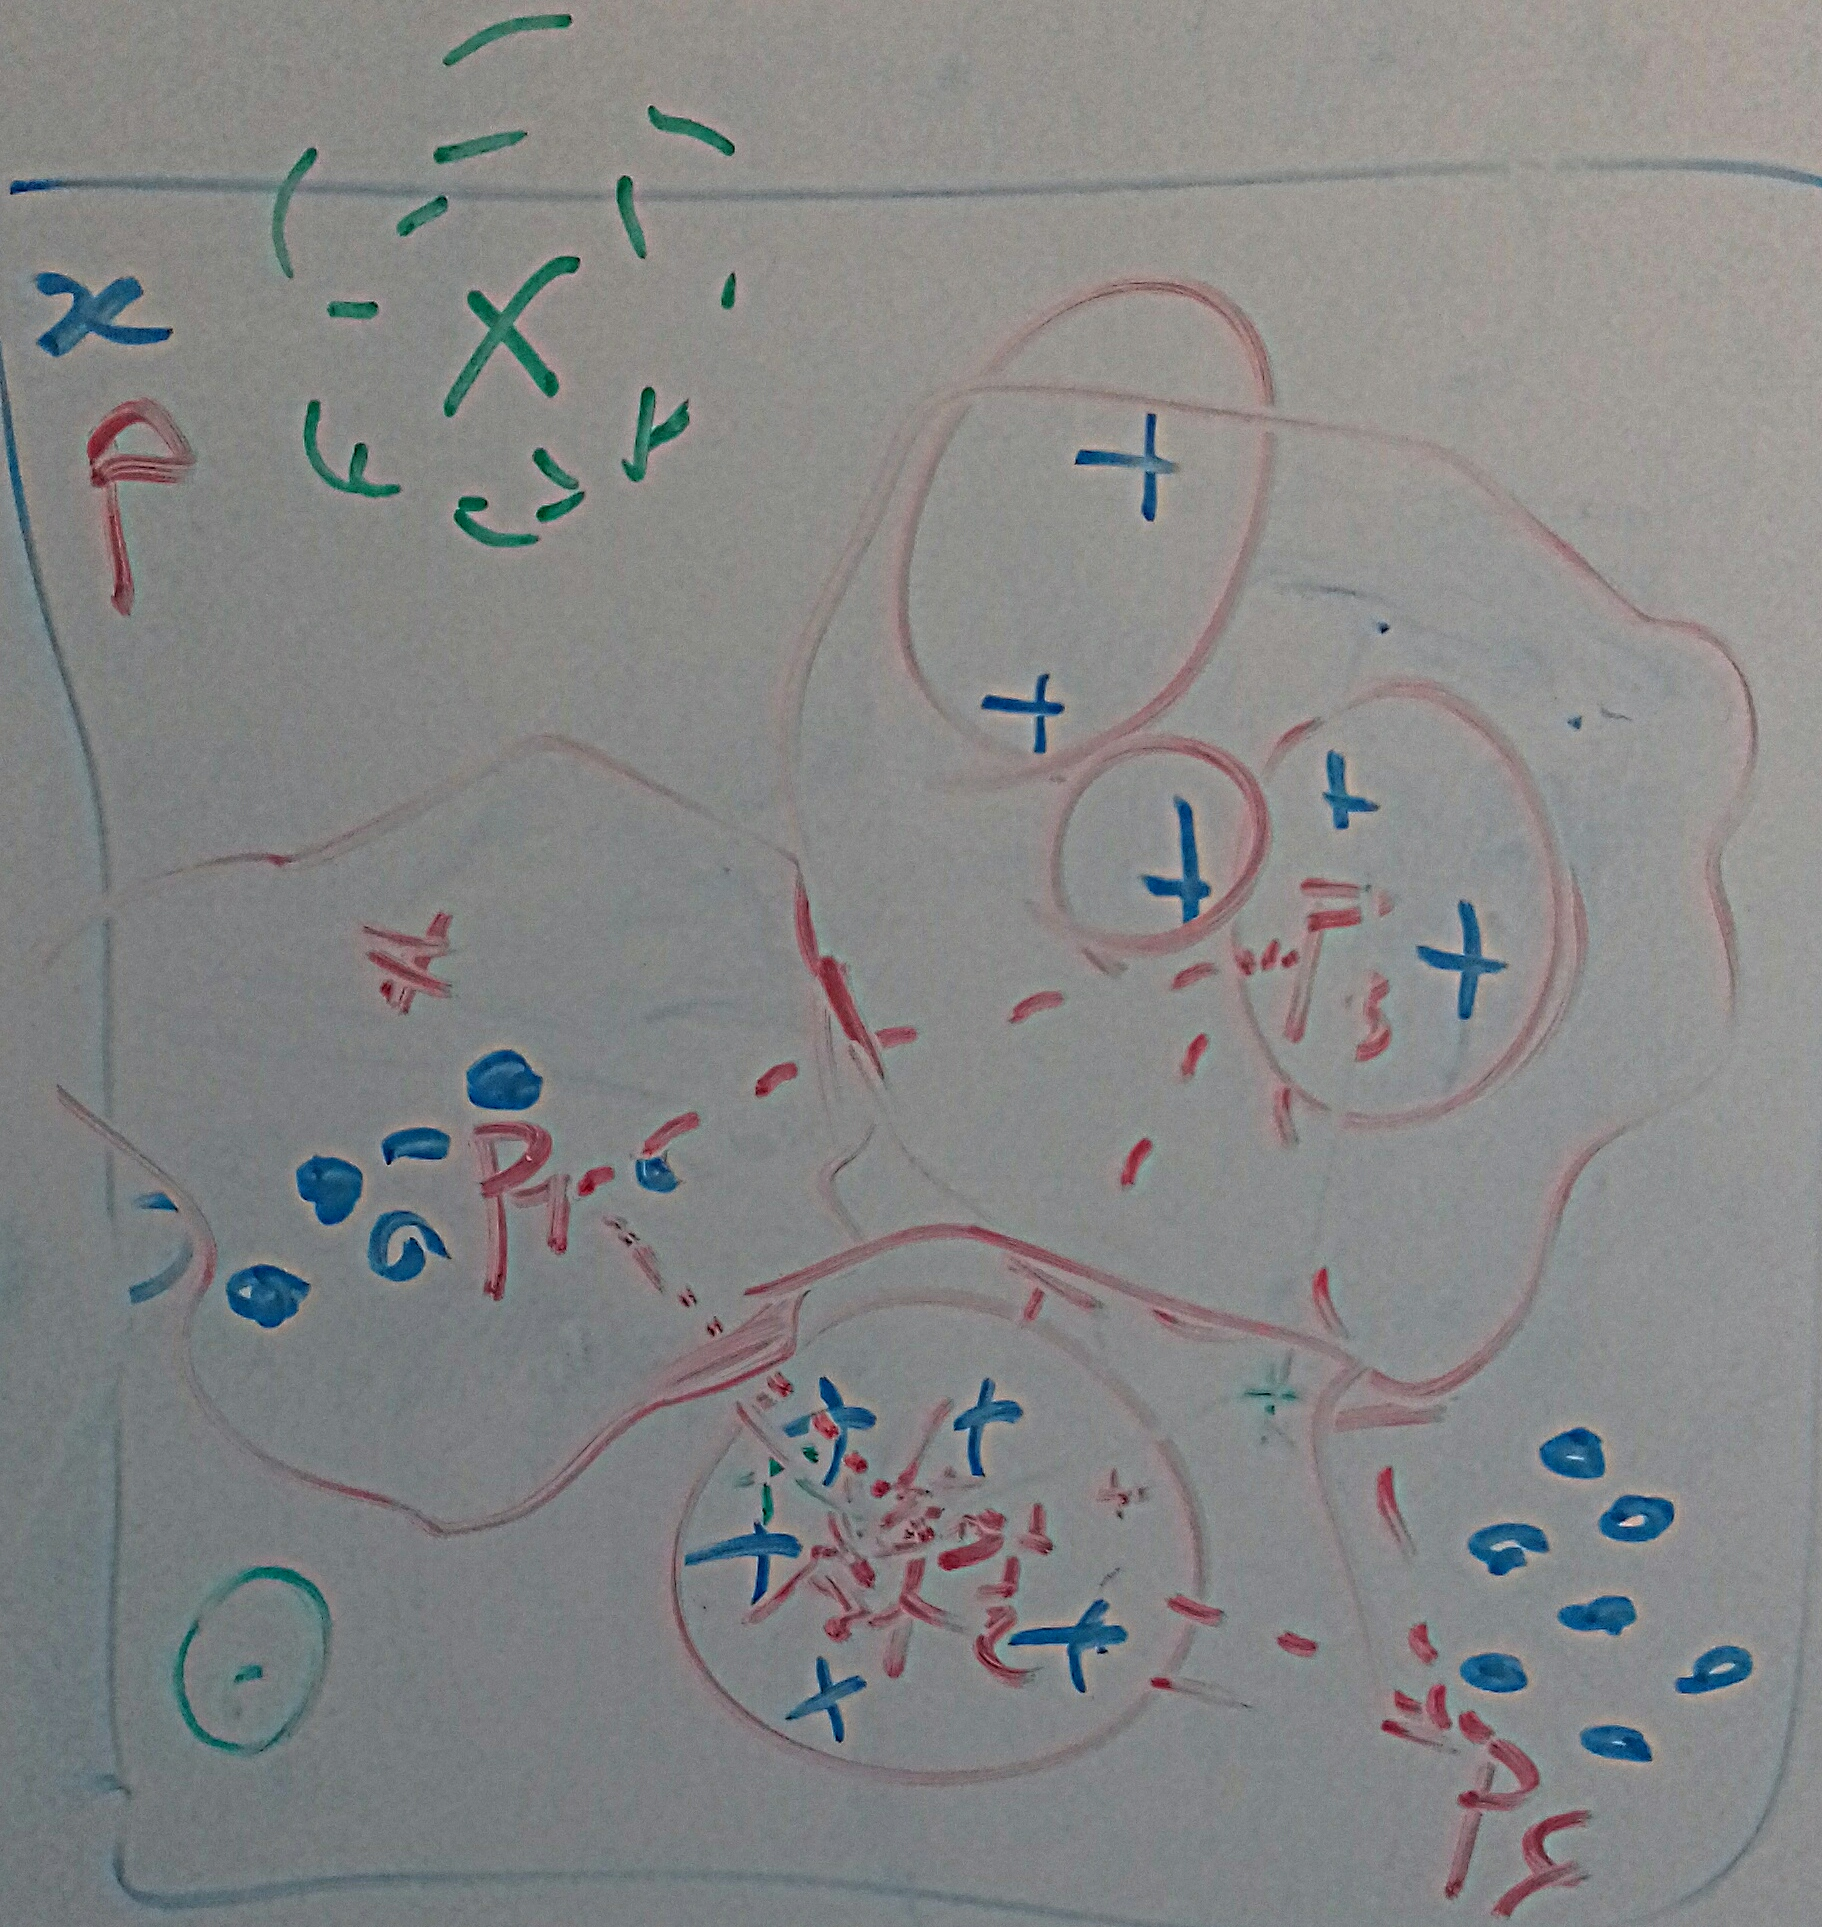
\includegraphics[width=0.8\textwidth,height=5cm]{img/20170920_163743}\end{center}

The task here is discrimination. So what ?

\subsection*{Adding a TFD (Twisted Features Discriminator) layer}

In order to improve existing methods, here, we introduce the notion of prototype in order to discriminate between twisted features at the output of some convolutional deep learning layers and before the usual softmax classifier, as shown here:

\begin{center}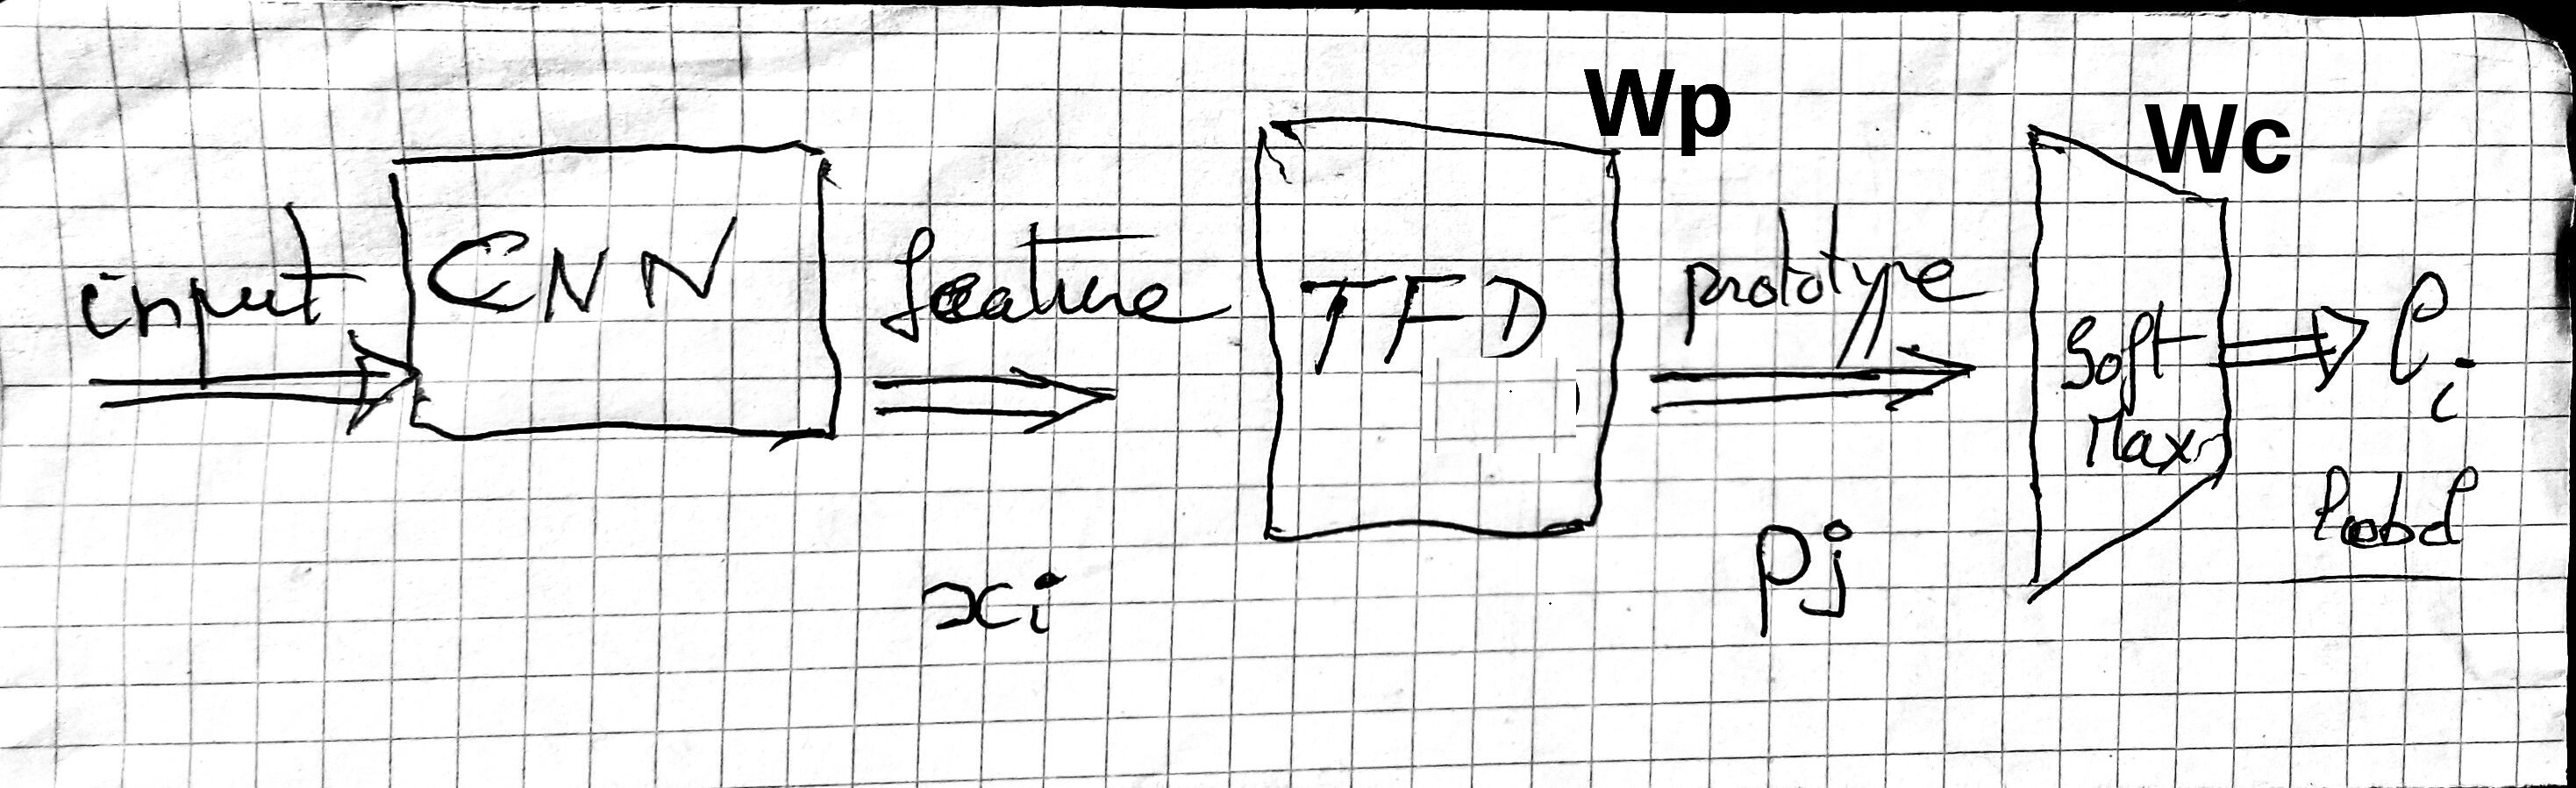
\includegraphics[width=0.8\textwidth]{img/20170923_114401}\end{center}

The key ideas are that the TFD is going to both \\ - (i) being able to identify different unconnected or twisted regions of the feature space related to the same labeled category (i.e., take into account the fact that the feature space is twisted with respect to the category labels) and also \\ - (ii) correctly represent small-shot, one-shot or zero-shot category by some prototype (or absence of prototype) learned on a very few number of samples.

To this end, we propose to consider the estimation of a fixed-size set of prototypes in the feature space ${\bf p}_j$, $j \in \{0, J\}, J  \geq L$, in order, as far as classification is concerned, to approximate the features by these prototypes and estimate:
\\ \tab -1- On one hand, $q_j({\bf x}) = p({\bf p}_j \in Q_j | {\bf x})$ is the probability for a feature vector, a sample ${\bf x}$, to be associated to the $j$-th prototype. \vthierry{This association is represented by the relation ${\bf p}_j \in Q_j$, in words: The fact that the sample belongs to the set of sample associated to the given prototype.}
\\ \tab -2- One the other hand, $c_{l}({\bf x}) = p(l | {\bf x})$ is the probability for a sample to be associated to the label of index $l$,
\\ this corresponding to both TFD and SoftMax layers parameterized by ${\bf W_p}$ and ${\bf W_c}$ respectively.

A step further, 
\\ \tab -1- we approximate $q_j({\bf x})$ by softmax layer \vthierry{idée issue du papier de [euh quel papier :) ?]}, that computes the probability as a function of the distances $\|{\bf x} - {\bf p}_j\|$ to the prototypes, writing:
\eqline{\begin{array}{rcll} q_j({\bf x})
&\deq& {}_{\tau}\nu_j\left(-\|{\bf x} - {\bf p}_j\|^2/2\right) \\
&=& {}_{\tau}\nu_j\left({\bf p}_j^T\,{\bf x} - \|{\bf p}_j\|^2/2 -  \|{\bf x}\|^2/2\right) & \mbox{by expansion}\\
&=& {}_{\tau}\nu_j\left({\bf p}_j^T\,{\bf x} - \|{\bf p}_j\|^2/2\right) & \mbox{by offset invariance}\\
\end{array}}
using the softmax function:
\eqline{{}_\tau\nu_j\left({\bf x}\right) \deq \frac{\exp(f_j({\bf x})/\tau)}{\sum_{j'} \exp(f_{j'}({\bf x})/\tau)}}
writing\footnote{\vthierry{More generally we can consider $f_j({\bf x}) \deq -\|{\bf x} - {\bf p}_j\|^d/d$, yielding $\partial_{{\bf p}_j} f_j({\bf x})*T = \|{\bf x} - {\bf p}_j\|^{d-2}\, ({\bf x} - {\bf p}_j)$, in order to deal with more than the ${\cal L}^2$ norm (e.g., for sparse estimation).}} $f_j({\bf x}) \deq {\bf p}_j^T\,{\bf x} - \|{\bf p}_j\|^2/2$, thus $\partial_{{\bf p}_j} f_j({\bf x})^T = {\bf x} - {\bf p}_j$ (see Appendix A for a review). The $N \times J$ ($N$ rows, $J$ columns) weight matrix ${\bf W}_{\bf p}$ corresponds to prototypes coordinates in the feature space.
\\ \tab -2- and we then approximate $c_l({\bf x})$ by another softmax layer
\eqline{\begin{array}{rcll} c_l({\bf x})
&\deq& {}_{\tau}\nu_l\left({\bf w}_l^T \, {\bf q}({\bf x})\right) \\
\end{array}} for some weights ${\bf w}_l$, which correspond to $J \times L$ weight matrix ${\bf W}_{\bf c}$. \vthierry{See Appendix B for the probabilistic interpretation of this formulation.}

\subsection*{Defining cross-entropy over both layers}

Considering an approximate cross-entropy criterion to adjust the parameters given samples ${\bf x}_i$ and their label $l_i$ yields the following minimization:
\eqline{\begin{array}{rcll} {\cal C} 
&=& -\int_{\cal X} p({\bf x}) \, \log\left(c({\bf x})\right) \\
&\simeq& -\frac{1}{N} \sum_{i} \log\left(c_{l_i}({\bf x}_i)\right) & \mbox{approximating $p()$ on the data samples} \\
\end{array}}
\vthierry{yielding:
\eqline{\begin{array}{rcll}
-N \, \tau \, \partial_{{\bf w}_{l}} {\cal C}^T &=& \sum_i \underbrace{\left[\delta_{l = l_i} - c_l({\bf x}_i)\right]}_{\alpha_i} \, {\bf q}({\bf x}_i) \\
-N \, \tau \, \partial_{{\bf p}_{j'}} {\cal C}^T &=&  \sum_i
\underbrace{\left[
\sum_j \left(w_{l_ij} - \sum_l c_l({\bf x}_i) \, w_{lj}\right) \, q_j({\bf x}_i) \, \left(\delta_{j = j'} - q_{j'}({\bf x}_i)\right)\right]}_{\beta_{ij'}} & ({\bf x}_{i} - {\bf p}_{j'}) \\
\end{array}}
} so that we can write, for some sufficiently small $\epsilon$:
\eqline{\Delta {\bf w}_l = \epsilon \sum_i \alpha_{i}  \, {\bf q}({\bf x}_i)
\mbox{ and }
{\bf p}_j = \sum_j \beta_{ij} \, {\bf x}_{i} / \sum_j \beta_{ij}}
at each step, and leading to:
\\ - expectation (estimated the prototypes as weighted mean over the samples), 
\\ - minimization (decreasing the criterion by adjusting the softmax weights) mechanism.

With such an approach there is no ``magouille''for better or for worse, while only a weak clustering of the samples with respect to a prototype, e.g., samples with different labels can be related to the same prototype. 

Initialization can be defined in two steps, using a deterministic or random version of the kmeans++ heuristic:
\\ -1- The 1st prototype is chosen, say, ${\bf p}_{j=0} = {\bf x}_{i=0}$, or at random, then for all other prototypes we choose the distant, which is the more distant to other prototypes, i.e.:
\eqline{\forall j \in \{1, J\{, {\bf p}_{j} = {\bf x}_{\mbox{arg min}_{i}, \max_{j' \in \{0, j\{} q_{j'}({\bf x}_i)},} or at random with a probability proportional to this.
\\ -2- Given prototypes initialization, we can compute each $l_j$ as below, and assume the classification is perfect:
\eqline{w_{lj} = \delta_{l = l_j}.}

% https://en.wikipedia.org/wiki/K-means_clustering#Standard_algorithm
% https://en.wikipedia.org/wiki/K-means%2B%2B#Improved_initialization_algorithm

\subsection*{Introducing information on the clustering}

We now also consider (as detailed in Appendix A):
\eqline{q({\bf x}_i) = \sum_j p({\bf x}_i \in P_j) \, p({\bf p}_j|{\bf x}_i) = \sum_j  \kappa_{ij} \, q_j({\bf x}_i)}
thus new parameters $\kappa_{ij} \deq p({\bf x}_i \in P_j)$ defining the clustering, i.e., the fact that a given sample belongs to a cluster.

During the learning phase both the ${\bf p}_j$ values and the $\kappa_{ij}$ are adjusted, after the learning phase, only ${\bf p}_j$ are used.

Given the samples ${\bf x}_i$ and the label $l_i$ we can easily define the maximum likelihood\footnote{\vthierry{we can write:
\eqline{\begin{array}{rcll} l_j 
&=& \max_l p(l|{\bf p}_j) & \mbox{as maximum likelihood} \\
&=& \max_l \int_{\bf x} p(l,{\bf x}|{\bf p}_j) & \mbox{writing it as marginalization on the data} \\
&=& \max_l \int_{\bf x} p(l,{\bf p}_j|{\bf x}) \, p({\bf x}) / p({\bf p}_j)& \mbox{from Bayses' rule} \\
&=& \max_l \int_{\bf x} p(l,{\bf p}_j|{\bf x}) \, p({\bf x})& \mbox{since $p({\bf p}_j)$ is constant with respect to the max} \\
&=& \max_l \sum_i p(l,{\bf p}_j|{\bf x}_i) & \mbox{sampling on the learning set} \\
&=& \max_l \sum_i \delta_{l = l_i} p({\bf p}_j|{\bf x}_i) & \mbox{since label $l_i$ is given for each ${\bf x}_i$} \\
&=& \max_l \sum_{i, l = l_i} q_j({\bf x}_i) & \mbox{by a simple change of notation} \\
\end{array}}}} of a category:
\eqline{l_j = \mbox{arg max}_{l} \sum_{i, l = l_i} q_j({\bf x}_i).}


The strong constraint is that the samples $({\bf x}_i, l_i)$ being labeled, only samples with the {\em same} label $l_j$, can be associated to a given prototype ${\bf p}_j$, $l_i \neq l_j \Rightarrow \kappa_{ij} = 0$.

This can be implemented in two steps:
\\ \tab -1- Initialize $\kappa_{ij} = q_j({\bf x}_i)$, and calculate $l_j$, as above.
\\ \tab -2- Resets all $\kappa_{ij}$ such that $l_i \neq l_j$, and re-normalize $\kappa_{ij}$.

Furthermore:

- For a ``lonely'' sample with all $\forall j, \kappa_{ij} = 0$, it means that it is not associated to a prototype and a new prototype has to be taken into account (initialized with ${\bf p}_j = {\bf x}_i$ and $\kappa_{ij} = \delta_{i = j}$).

- Unused prototypes correspond to the situation with $\forall i, \kappa_{ij} = 0$.

- Given a prototype ${\bf p}_j$ such that $\forall i, \kappa_{ij} \leq \max_{j', j' \neq j} \kappa_{ij'}$ (i.e., for which samples are all better represented by other prototypes) can be set as unused, i.e. with $\forall i, \kappa_{ij} = 0$. \vthierry{This condition qualitatively corresponds to isolated prototypes, i.e. such stat each sample is closer to another prototype.}

\vthierry{- If a new prototype is required, for a lonely sample, and no unused prototype is available, we must delete a used prototype ${\bf p}_{j^\dagger}$, and the choice is to be done: 
\\ \tab - among prototypes that do not generate a lonely sample, i.e. $\forall i, \kappa_{ij^\dagger} > 0, \exists j, \kappa_{ij} > 0$. If all prototypes delete generate lonely sample, this means that algorithm fails, in fact that there is more label than prototypes, but we choose $J \geq L$.
\\ \tab - considering the prototype that minimize the increase of the distance from sample to prototypes, i.e.:
\eqline{j^\dagger = \mbox{argmin}_j \, \max_i \, \left(\kappa_{ij} - \max_{j', j' \neq j} \kappa_{ij'} \right),}
in words, the prototype for which the maximal distance increase yielded by replacing this prototype by the best other one is minimal. \vthierry{Ouille, é necessário retomar a respiração para seguir esse objetivo!} [something more simple ?]
}

\subsection*{Defining cross-entropy for the TFD layer}

Considering an approximate cross-entropy criterion to adjust the prototypes yields the following minimization:
\eqline{\begin{array}{rcll} {\cal C} 
&=& -\int_{\cal X} p({\bf x}) \, \log\left(q({\bf x})\right) \\
&\simeq& -\frac{1}{N} \sum_{i} \log\left(q({\bf x}_i)\right) & \mbox{approximating $p()$ on the data samples} \\
&=& -\frac{1}{N} \sum_{i} \log\left(\sum_j \kappa_{ij} \, q_j({\bf x}_i)\right) & \mbox{from the previous statement}\\
&=& -\frac{1}{N} \sum_{i} \log\left(\sum_j \kappa_{ij} \, {}_{\tau}\nu_j\left({\bf p}_j^T\,{\bf x}_i - \|{\bf p}_j\|^2/2\right)\right) & \mbox{by substitution}\\
\end{array}}
yielding:
\eqline{-N \, \tau \, \partial_{{\bf p}_{j'}} {\cal C}^T = \sum_{i} \mu_{ij'} \, ({\bf x}_i - {\bf p}_{j'}),\;\;\;  \mu_{ij'} \deq \hat{\mu}_{ij'} - q_{j'}({\bf x}_i),\;\;\; \hat{\mu}_{ij'} \deq \frac{\kappa_{ij'} q_{j'}({\bf x}_i)}{q({\bf x}_i)} }
providing a weighted estimation of the prototypes, $\partial_{{\bf p}_{j'}} {\cal C}^T = 0$ yields:
\eqline{{\bf p}_{j'} = \sum_i \mu_{ij'} \, {\bf x}_i \left/ \sum_i \mu_{ij'} \right.}
as a function of $q_{j'}({\bf x}_i) = p({\bf p}_{j'}|{\bf x}_i)$ and $\hat{\mu}_{ij'} = p({\bf x}_i|{\bf p}_{j'})$.

\clearpage \appendix \section*{A few more details}

\subsection*{A - The softmax function and its estimation}

The softmax function generalizes the logistic function and enjoys the facts that:
\eqline{0 \leq {}_\tau\nu_j\left({\bf x}\right) \leq 1,\; \sum_j {}_\tau\nu_j\left({\bf x}\right) = 1,\; \left.{}_\tau\nu_j\left({\bf x}\right)\right._{f_j \rightarrow f_j + o} = {}_\tau\nu_j\left({\bf x}\right),\; {}_{\tau/\tau'}\nu_j\left({\bf x}\right) = {}_\tau\nu_j\left({\bf x}\right)^{\tau'} \left/ \sum_{j'} \nu_{j'}\left({\bf x}\right)^{\tau'} \right.,}
in words, probabilities with offset invariance and power effect of the temperature $\tau$, while:
\eqline{{}_\tau\nu_j\left({\bf x}\right) = \left.\max_j(f_j({\bf x}))\right._{\tau \rightarrow o} = \frac{1}{J} + \frac{1}{\tau\, J} \, \left( f_j({\bf x}) - \frac{1}{J} \, \sum_{j'} f_{j'}({\bf x}) \right) + O\left(\frac{1}{\tau^2}\right),}
computes the maximal values at low temperature, while approximating the given affine operator at high temperature. 
% maple line to get the previous formula: series(exp(k*z[0])/(exp(k*z[0])+sum(exp(k*z[i]),i=1..J-1)), k = 0, 2); 
A step further, for some parameter $\theta_{j'}$ of the $f_{j'}({\bf x})$ we obtain:
\eqline{\tau \, \partial_{\theta_{j'}} {}_\tau\nu_j({\bf x}) = {}_\tau\nu_j({\bf x}) \, (\delta_{j = j'} - {}_\tau\nu_{j'}({\bf x})) \, \partial_{\theta_{j'}} f_{j'}({\bf x}),}
while for some parameter $\theta$ of the ${\bf x}$ we obtain:
\eqline{\tau \, \partial_{\theta} {}_\tau\nu_j({\bf x}) = {}_\tau\nu_j({\bf x}) \, \left(\partial_{\bf x} f_{j}({\bf x}) - \sum_{j'} {}_\tau\nu_{j'}({\bf x}) \, \partial_{\bf x} f_{j'}({\bf x})\right) \,  \partial_{\theta} {\bf x}.}

Considering an approximate cross-entropy criterion to adjust the values of a standard softmax criterion yields the following minimization:
\eqline{\begin{array}{rcll} {\cal C} 
&=& -\int_{\cal X} p({\bf x}) \, \log\left(\nu({\bf x})\right) \\
&\simeq& -\frac{1}{N} \sum_{i} \log\left(\nu({\bf x}_i)\right) & \mbox{approximating $p()$ on the data samples} \\
&=& -\frac{1}{N} \sum_{i} \log\left(\nu_{l_i}({\bf x}_i)\right) & \mbox{since each sample is associated to one class} \\
&=& -\frac{1}{\tau\,N} \sum_{i} f_{l_i}({\bf x}_i) + \log\left(\sum_{j'} \exp(f_{j'}({\bf x})/\tau)\right) & \mbox{by substitution and factorization} \\
\end{array}}
yielding the gradient, for a parameter $\theta_{j'}$ of the function $f_{j'}({\bf x})$:
\eqline{-\tau \, \partial_{\theta_{j'}} {\cal C} = \left( \frac{1}{N} \sum_i \delta_{j' = l_i} - {}_\tau\nu_{j'}({\bf x}) \right) \, \partial_{\theta_{j'}} f_{j'}({\bf x}).}

%ref: http://peterroelants.github.io/posts/neural_network_implementation_intermezzo02/

\subsection*{B - Probabilistic interpretation of representing samples by prototypes}

Representing the sample ${\bf x}$ by prototypes means approximating the ${\bf x}$ distribution by a distribution only function of the prototypes, e.g.:
\eqline{{\bf x} \simeq \mathbb{E}_{\hat{q}}({\bf x}) = \sum_j q_j({\bf x}) \, {\bf p}_j, \mbox{ with } \hat{q}({\bf x}) \deq \sum_j q_j({\bf x}) \, \delta({\bf x} - {\bf p}_j)}
where $\hat{q}({\bf x})$ approximates the true sample probability distribution $p({\bf x})$ as a discrete distribution, given the prototypes. 

Another view is to consider a partition $\{\cdots, P_j, \cdots\}$ of the space induced by the prototypes (i.e., with ${\bf p}_j \in P_j$, see Appendix C), yielding:
\eqline{q({\bf x}_i) = \sum_j p({\bf x}_i \in P_j) \, p({\bf p}_j|{\bf x}_i) = \sum_j  \kappa_{ij} \, q_j({\bf x}_i)}
for some $\kappa_{ij} = p({\bf x}_i \in P_j)$. Here the partition has not to be made explicit, only the $\kappa_{ij}$ have to be estimated. We notice that:
\\ - We obtain $\sum_j \kappa_{ij} = 1$ (since $P_j$ forms a partition).
\\ - The $\kappa_j \deq \sum_i \kappa_{ij}$ is the expectation of the number of sample in the partition, i.e. associated to the prototype. 
\\ - If $\kappa_j = 0$ the prototype is inactive, i.e., not associated to any sample. 
\\ - If $\kappa_{ij} \in \{0, 1\}$, i.e, if we know whether ${\bf x}_i \in P_j$ or not, i.e., is related to this prototype or not, 
\\ \tab - the constraint $\sum_j \kappa_{ij} = 1$ states that each sample is associated to a unique prototype, 
\\ \tab - while $\kappa_j \deq \sum_i \kappa_{ij}$ is the number of samples associated to a given prototype. 

\vthierry{A step further, the fact we consider for $c_l({\bf x})$:
\eqline{p(l|{\bf x}) = {}_{\tau}\nu_l\left({\bf w}_l^T \, p({\bf p}_j \in Q_j | {\bf x})\right) \neq \sum_j p(l|{\bf p}_j \in Q_j) \, p({\bf p}_j \in Q_j | {\bf x})}
simply means that we do {\em not} consider that the $Q_j$, namely the set of sample associated to a the $j$-th prototype, corresponds to a partition of the sample space ${\cal X}$, but that the corresponding regions may overlap, while some regions may not correspond to sample associated to any prototypes.}

\subsection*{C - Duality between partition, prototypes and metric}

Given a set of prototypes ${\bf P}=\{\cdots{\bf p}_j\cdots\}$ in a topological space ${\cal X}$ we can consider a  partition of the space $P = \{\cdots{P}_j\cdots\}$ around the prototypes, i.e. such that
\eqline{{\bf p}_j \in P_j \neq \emptyset,\;\;\; \cup_j P_i = {\cal X}, \;\;\; \forall i,j, \mathring{P}_j \cap \mathring{P}_i = \emptyset.}
The last condition means that we do not require the intersection to be empty but only its interior (i.e., maximal open set). This notion of partition is thus related to a topology. Roughly speaking, this means that we do not take into account what happens at the frontier between two subsets of the partition. 
For any point, but those at the frontier between two subsets, we can define its partition subset index $j = p({\bf x}) = \{j, {\bf x} \in P_j\}$.

Given a set of prototypes, any metric induces such a partition, writing:
\eqline{P_j = \{ {\bf x} \in {\cal X}, d({\bf x}, {\bf p}_j) <= min_{j'} d({\bf x}, {\bf p}_{j'}) \}}
On the reverse, given a partition and a topology, the ultrametric:
\eqline{d({\bf x}, {\bf y}) = \delta_{{\bf x} \neq {\bf y}} \, (1 + \delta_{p({\bf x}) \neq p({\bf y})}) \in \{0, 1, 2\}}
is a trivial metric compatible with the partition (i.e. fitting in the previous definition).

More interesting is the fact that given any partition with a metric, and choosing a precision $\epsilon$ there exists a countable set of prototypes such that the given partition is a subset of the partition induced by these prototypes, up to the $\epsilon$ precision. If ${\cal X}$ is bounded, e.g. compact, the prototype set if finite. Let us consider this case. Any compact set has always a finite cover. As being a metric space, it always has a finite cover by balls of a given radius, say $B({\bf p}_i, \epsilon/2)$. From this construction, we only keep the prototypes corresponding to the center of balls that intersect the initial partition subsets frontiers. It is then easy to prove that this induce, up to $\epsilon$, a partition:
\eqline{{\bf p}_j \in P_j \neq \emptyset,\;\;\; \cup_j P_i = {\cal X}, \;\;\; \forall i,j, P_j \cap P_i \subset B({\bf p}_i, \epsilon),}
where $P_j$ is defined from the metric as given above. Such a construction is related to vector support machines, the given prototypes being somehow the classification support set.

\iffalse
\subsection*{C - Inferring a probability distribution}

Given a set of samples ${\bf x}$ inferring the related probability distribution is a ill-defined and intractable problem in the general case, but it is interesting to consider a maximal entropy distribution coherent with the sampling in the following sense:
\eqline{ \int_{{\cal V}_k \subset {\cal X}}  p({\bf x}) = \frac{1}{N} \, \sum_{i, {\bf x}_i \in {\cal V}_k} 1}
for some neighborhood ${\cal V}_k$ of the samples, i.e., 
\eqline{p = \mbox{arg max}_p \int_{\cal X} p({\bf x}) \, \log\left(p({\bf x})\right) + 
 \lambda_0 \left( \int_{\cal X} p({\bf x}) - 1 \right) +
 \sum_k \lambda_k \, \left( \int_{{\cal V}_k \subset {\cal X}}  p({\bf x}) - \frac{1}{N} \, \sum_{i, {\bf x}_i \in {\cal V}_k} 1 \right)}
, yielding:
\eqline{p({\bf x}) = \frac{1}{Z({\bf \lambda})} \, \exp\left(\sum_k \lambda_k \, \mathbf{1} _{{\cal V}_k}({\bf x})\right).}
We likely can further require the distribution to be regular, vanishing at infinity, increasing ... 
\fi

\end{document}
